\chapter{环境与认知的结构对应：可观测性与近似等价}
\label{chp:holomorphic_isomorphism}
% Compatibility anchors: old section references resolve to this chapter.
\label{sec:brain_cosmos}
\label{sec:holomorphic_theorem}
\label{sec:comprehensibility}
\label{sec:godel_gap}

我们将环境与内部模型的关系表述为任务相关的结构对应。预测性能可以约束内部表示，但不能单独证明内部空间与整个环境同胚。
\section{任务相关的等价类}
令环境状态为 $z$，允许的动作和观测历史共同确定任务。若两状态在所有允许策略下产生相同的未来任务观测分布，我们将它们记为 $z\sim z'$。这个等价关系依赖任务、传感器和可用干预；改变这些条件后，原等价类可能需要细分。
\section{动力学映射的定义}
考虑确定性特例 $z_{k+1}=T(z_k,a_k)$，内部状态 $x=e(z)$，内部预测转移为 $\widehat T$。严格对应要求
\begin{equation}e(T(z,a))=\widehat T(e(z),a).\end{equation}
这是转移的交换关系。如果 $e$ 非单射，它至多构成任务相关的压缩映射；只有补充双射、逆映射的连续性等条件，才能讨论同胚。随机系统须比较转移核而非单个状态点。
\section{近似误差的传播}
设编码域内的一步误差不超过 $\delta$，$\widehat T$ 对状态为 $L$-Lipschitz，且比较轨迹使用同一动作序列。令 $E_k=\|e(z_k)-x_k\|$，三角不等式给出 $E_{k+1}\le\delta+LE_k$。若 $E_0=0$，则
\begin{equation}E_k\le\delta\sum_{j=0}^{k-1}L^j.\end{equation}
当 $L<1$ 时误差有统一上界；$L\ge1$ 时长期误差可能增长。闭环动作随内部预测改变时，还需计入策略敏感性。本书据此将结构对应视为有条件、可测量的模型性质。

\section{表示与示意图}
我们保留以下示意图以展示原有结构关系。图中历史物理术语遵循阅读约定中的计算解释；图的形式相似性不代替本章的假设、推导和验证。
\begin{figure}
\centering
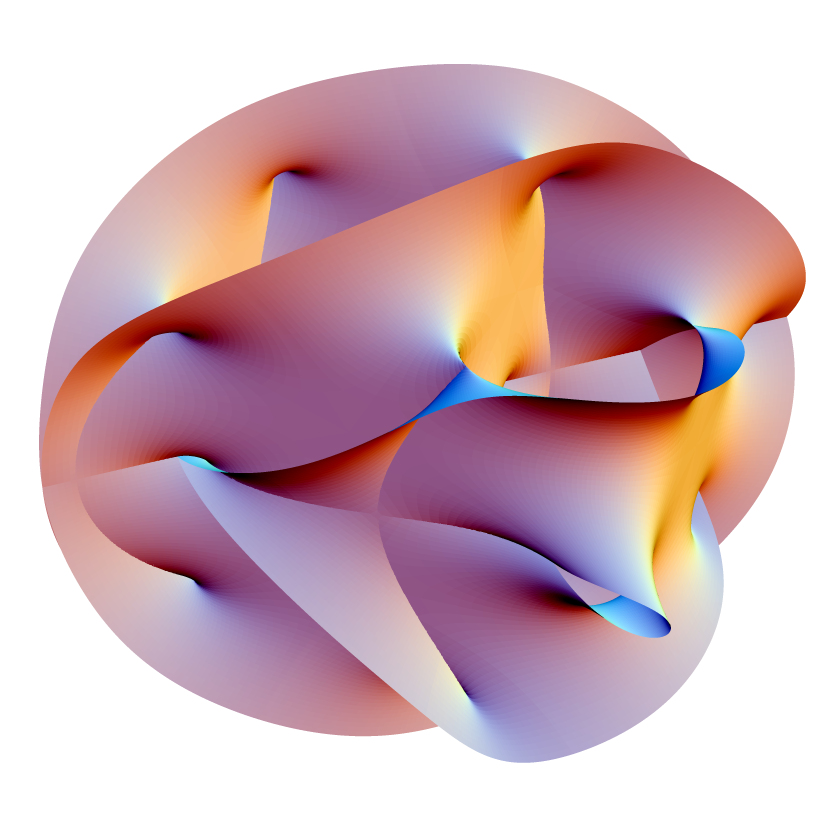
\includegraphics[width=0.4\textwidth]{image/Calabi.png}
\caption{一种流形结构}
\end{figure}

